% SPDX-FileCopyrightText: 2023 SAP SE
%
% SPDX-License-Identifier: Apache-2.0
%
% This file is part of FEDEM - https://openfedem.org

%%%%%%%%%%%%%%%%%%%%%%%%%%%%%%%%%%%%%%%%%%%%%%%%%%%%%%%%%%%%%%%%%%%%%%%%%%%%%%%%
%
% FEDEM User Guide.
%
%%%%%%%%%%%%%%%%%%%%%%%%%%%%%%%%%%%%%%%%%%%%%%%%%%%%%%%%%%%%%%%%%%%%%%%%%%%%%%%%

\Section{Parts}{parts}

As described in \refChapter{introduction-to-fedem}{Introduction to Fedem},
{\sl parts} are the basic components of Fedem models. You can connect parts
with various types of joints to create a movable mechanism.
Each part is either an {\sl FE Part} represented by a standard FE model,
or a {\sl Generic Part} represented by a simplified model forming a semi-rigid
connection between other mechanism entities.

Two-noded beams may also be used in place of parts when constructing
a Fedem model. A beam is somewhat equivalent to a Generic Part connected
to two triads, except that the mass- and stiffness matrices are derived
consistently from a linear beam finite element,
instead of using the semi-rigid representation.
Such elements are denoted {\sl Beams} in the Model Manager and are described in
\refSection{beams}{Beams}.


\subsubsection{FE Parts}

The mass-, stiffness- and dynamic properties of an FE Part are defined
through its FE model, defined by nodes, elements, materials and physical
property data. The FE model must be constructed in an external FE modeler,
such as one of those described in \refSection{using-fe-models}{Using FE models},
and then imported into Fedem.

You can use simple or complex parts in your models, depending on your needs and
modeling capabilities.
Shown below is a simple FE part modeled with solid elements.

\noindent
\begin{minipage}{0.57\textwidth}
  \raggedright
  \begin{bulletlist}
    \setlength\itemsep{2mm}
  \item{\sl Part coordinate system} --
    The FE model representing the part is defined in the part coordinate system.
    When the part is imported into Fedem this coordinate system is aligned with
    the global coordinate system.
  \item{\sl Triads} (optional) --
    nodal points that are defined as external during the construction of an
    FE model in an external modeler, are connected to automatically generated
    triads when the part is imported into Fedem.
  \end{bulletlist}
\end{minipage}% <--- the % is needed here to kill off spurious spacing
\hfill\begin{minipage}{0.4\textwidth}
  \begin{picture}(140,150) % 4-Link-sec-4.2.bmp
    \put(0,0){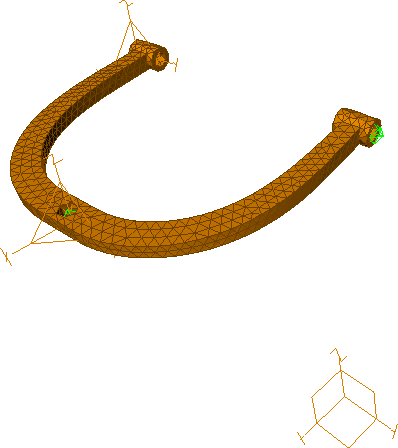
\includegraphics[width=\textwidth]{Figures/4-horseshoe}}
    \put(112,3){\Bullet{1}}
    \put(131,100){\Bullet{2}}
    \put(10,58){\Bullet{3}}
    \put(30,140){\Bullet{3}}
  \end{picture}
\end{minipage}

\MiniGenericNote{note}{NOTE}{-25mm}{1.1}{0.157}{0.843}{
  If external nodes are not defined in the FE model file, no triads will
  appear when the model is imported (see \refSection{triads}{Triads}
  for more information about triads).}

\begin{bulletlist}
  \setcounter{enumi}{2}
\item{\sl Local coordinate systems} --
  Local FE coordinate systems present in the imported FE model
  is read and displayed for reference.
\end{bulletlist}


\subsubsection{Generic Parts}

A Generic Part is a simplified flexible body. It is purely defined by
its connection points, mass properties and stiffness at the connection
points. The stiffness can either be defined manually, or automatically
set to some very high value, mimicking a rigid body.
See the \FedemTGuide{Section A.16, "Generic Part element"}, for details
on how a Generic Part is represented in the Dynamics Solver.

\Tip{
  As an alternative to using Generic Parts, entirely user-defined elements may
  also included in you model. User-defined element types can be programmed
  according to a defined interface, and loaded into Fedem as a plugin.
  See \refSection{user-defined-elements}{User-defined elements}
  on how to implement your own set of user-defined elements.}

Generic Parts can be used when you have no FE model for the part, when
trying to optimize hard-point positions, or when the flexibility of the
part is considered to be insignificant. They can also have a VRML
geometry attached, to give better visualization of the part.

Shown below is a Generic Part with two triads and a Revolute Joint connected
to it.

\begin{figure}[H]
  \center
  \begin{picture}(265,95)
    \put(0,0){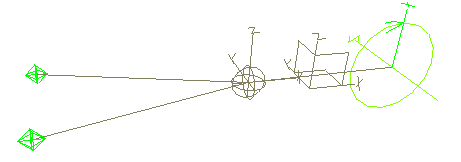
\includegraphics[width=0.8\textwidth]{Figures/generic-part}}
    \put(172,75){\Bullet{1}}
    \put(135,65){\Bullet{2}}
    \put(80,35){\Bullet{3}}
  \end{picture}
\end{figure}

\begin{bulletlist}
\item{\sl Part coordinate system} --
  At the time of creation, the part coordinate system is in the global origin.
\item{\sl Centre of Gravity} --
  The Generic Part's centre of gravity can be positioned independently
  from the part coordinate system.
\item{\sl Simplified visualization} --
  The lines extending from the centre of gravity to each of the triads attached
  provides a coarse visualization of the Generic Part.
\end{bulletlist}


%%%%%%%%%%%%%%%%%%%%%%%%%%%%%%%%%%%%%%%%%%%%%%%%%%%%%%%%%%%%%%%%%%%%%%%%%%%%%%%%
\SubSection{Visualization of beam element orientation and eccentricity in FE Parts}
           {visualization-of-beam-element-orientation-and-eccentricity-in-fe-parts}


For FE Parts containing beam elements, each beam element is represented
by a straight line connecting its two end nodes in the Fedem
{\sl Modeler} view. This is sufficient for elements with a circular cross
section where the properties will be independent of the element orientation.
However, for all non-circular cross sections some visualization of element
orientations is required to verify that the properties are correctly defined.
A full rendering of the actual cross section will provide such verification,
but this may result in a too big visualization model for FE Parts containing
a lot of beam elements. Instead,
Fedem provides a simplified visualization of the beam element orientation.

\begin{figure}[H]
  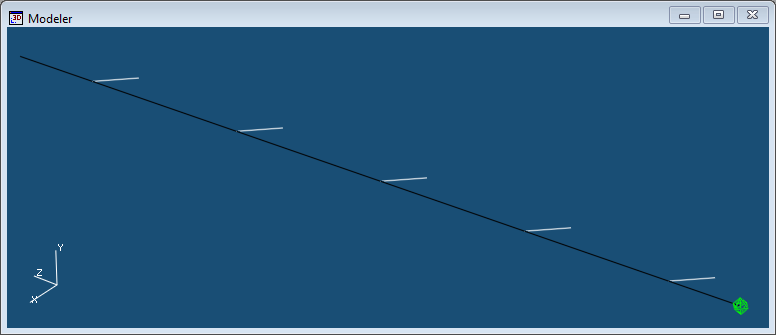
\includegraphics[width=\textwidth]{Figures/4-FEBeamOrient}
\end{figure}

The image above shows a simple FE part consisting of 5 beam elements and with
element orientation visualization activated.
It consists of a white line in the local XZ-plane of each beam element,
extending from the mid-point of each element towards local end 1 of the element
such that it forms a 45-degree angle with the local X-axis of the element.
The length of the orientation line is constant and independent of the element
length itself. Its length is scaled by the factor entered in the {\sl Size}
field in the General Appearance dialog box,
see \refSection{general-appearance}{General Appearance}.

The beam element orientation visualization is switched off by default.
To enable it, activate the {\sl Local coordinate systems} toggle in the
General Appearance dialog box,
see \refSection{general-appearance}{General Appearance}.

Beam elements may also have an eccentric coupling to the FE nodes.
The beam axis is in this case visualized in its eccentric position, and with
a white line connecting the eccentric beam end with the associated FE node.


%%%%%%%%%%%%%%%%%%%%%%%%%%%%%%%%%%%%%%%%%%%%%%%%%%%%%%%%%%%%%%%%%%%%%%%%%%%%%%%%
\SubSection{Creating parts by file import}{creating-parts-by-file-import}

Parts can be created by importing FE model files or by importing CAD
geometry as VRML files. The available file formats are listed in
\refSection{storing-models-and-results}{Storing models and results}.
Importing FE models will create an FE Part, while importing a VRML file
will create a Generic Part. In either case, complete the following steps,
to import a part:

\vskip\parskip
\IconText{loadLink}{\vskip-5mm
  \begin{itemize}
    \setlength\itemsep{1mm}
  \item[1.]
    Click the \textbf{Load Part} button on the \textbf{Mechanism Creation} tool
    bar (or select from the \textbf{File} menu). The dialog box shown below
    then opens.
    \begin{figure}[H]
      \center
      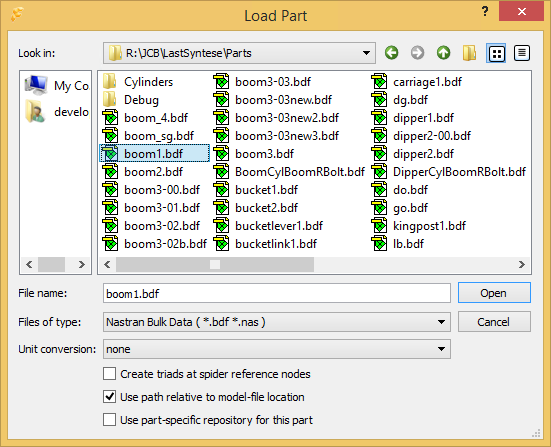
\includegraphics[width=0.8\textwidth]{Figures/Dialogs/4-LoadPart}
    \end{figure}
  \end{itemize}}

\begin{itemize}
\item[2.]
  Select the file type you want from the {\sl File of type} pull-down menu.

\item[3.]
  Browse for or type the path and name of the file in the {\sl File name} field.

\EnumTip{You can import more than one part at the same time by holding down
  the \textbf{Ctrl} or \textbf{Shift} key and selecting multiple files
  in the Load Part dialog box.}

\item[4.]
  Select the units conversion you need from the {\sl Unit conversion}
  pull-down menu. All units used in the file for dimensions and properties
  are converted according to your selection.

\EnumWarning{There is no connection between this unit conversion and the model
  database units. You must be careful to choose the conversion that fits
  your needs.}

\EnumTip{You can add your own unit conversions by editing the file
  \File{units.fcd} in any ASCII text editor.
   This file is located in the Fedem installation directory.}

\item[5.]
  If the FE model to be imported contains ``spider'' elements, i.e.,
  elements of types RGD or WAVGM (see
  \refSection{fedem-technology-link-format}{Fedem Technology Link format})
  or the Nastran elements RBE2 or RBE3 (see
  \refSection{nastran-bulk-data-file-format}{Nastran Bulk Data File format}),
  you may automatically create Triads at the
  reference nodes of these elements by enabling the toggle
  {\sl Create triads at spider references nodes}.

\item[6.]
  Make sure that you want to store the relative path to the original FE
  model or the VRML model. This setting is relevant when copying and
  moving the model across file systems, and has most impact on VRML
  files. The path to the original FE model file is only used if the
  internal FE model copies are lost.

\item[7.]
  Indicate if you want this part to be a part of the FE model
  repository, or if it should be stored with a part-specific repository.
  See \refSection{using-fe-model-repositories}{Using FE model repositories}.

\item[8.]
  Once you have selected the file(s) and a unit conversion, click \textbf{Open}.
  The part files are imported, and the coordinate system of the parts are
  aligned with the global coordinate system.
\end{itemize}

\begin{wrapfigure}{r}{0.3\textwidth}
  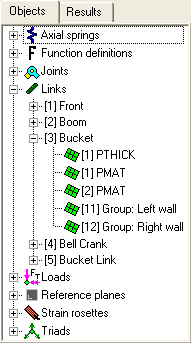
\includegraphics[width=0.3\textwidth]{Figures/4-ElementGroups}
\end{wrapfigure}

When an FE model is imported, it is converted to the internal Fedem format.
During this conversion, several
element groups might be created as well. These element groups can either
be user-defined explicit groups, or implicit groups based on the
properties of the elements in the FE part.

All element groups associated with a FE part are listed in the
{\sl Objects} list of the Model Manager panel, as illustrated to the
right. See \refSection{element-groups}{Element groups} to learn more
about element groups in Fedem.

\clearpage


%%%%%%%%%%%%%%%%%%%%%%%%%%%%%%%%%%%%%%%%%%%%%%%%%%%%%%%%%%%%%%%%%%%%%%%%%%%%%%%%
\SubSection{Creating parts from hard points}
           {creating-parts-from-hard-points}

If you only have the hard point information of a part, you can create a
part from triads positioned at the hard points as follows:

\vskip19mm
\IconText{genericPart}{\vspace*{-18mm}
  \begin{enumerate}
    \setlength\itemsep{1mm}
  \item
    Select the triads that represents the hard points of the part using
    the multi-select features of Fedem. See
    \refSection{model-manager}{Model Manager} and \refSection{select}{Select}
    on how to select multiple objects either from the {\sl Modeler} view
    or in the Model Manager {\sl Objects} list.
  \item
    Click the \textbf{Create Generic Part} button on the
    \textbf{Mechanism Creation} tool bar.
    A Generic Part will be created with its origin in the global origin, and
    with its centre of gravity in the geometric centre of the selected triads.
  \item
    Set up the centre of gravity and mass properties of the part.
  \item
    Optionally add more triads to the part by attaching them.
  \end{enumerate}}

\vskip-4mm
\Tip{You can at any time during modeling attach or detach
  new triads to the Generic Part.
  See \refSection{attaching-and-detaching-elements}
                 {Attaching and detaching elements}.}


%%%%%%%%%%%%%%%%%%%%%%%%%%%%%%%%%%%%%%%%%%%%%%%%%%%%%%%%%%%%%%%%%%%%%%%%%%%%%%%%
\SubSection{Copying parts}{copying-parts}

If you need to use the same FE model or Generic Part more than once,
you can duplicate an existing part by completing the following steps:

\vskip10mm
\IconText{copyLink}{\vspace*{-9mm}
  \begin{enumerate}
    \setlength\itemsep{1mm}
  \item
    Select the part you want to copy from the {\sl Modeler} view (or Model
    Manager {\sl Objects} list).
  \item
    On the \textbf{Edit} menu, select \textbf{Copy Part}.
\end{enumerate}}

\vskip-4mm
\noindent The new part is placed offset from the original.

\Tip{You can also copy parts using the shortcut menu in the Model Manager
  {\sl Objects} list. Right-click the part you want to copy and select
  \textbf{Copy Part} from the shortcut menu. The new part is placed offset
  from the original in the {\sl Modeler} view.}


%%%%%%%%%%%%%%%%%%%%%%%%%%%%%%%%%%%%%%%%%%%%%%%%%%%%%%%%%%%%%%%%%%%%%%%%%%%%%%%%
\SubSection{Part properties}{part-properties}

Parts are the basic components of any Fedem mechanism. It is therefore
essential to understand the part properties that are displayed in the
Property Editor panel when you select a part.

\Tip{In addition to the settings found in the Property Editor panel, you may
  also find some information on the part's underlying FE model by
  selecting the part in the Result File Browser (see
  \refSection{the-result-file-browser-dialog}{The Result File Browser dialog}).
}

The part properties are separated into several tabs to better organize
the different settings. The number of tabs and their content depend on
whether the part is defined as a Generic Part or an FE Part, or if it is
a part used for visualization only (grounded parts).

The different tabs are as follows:

\begin{itemize}
\item\protect\hyperlink{part-tab}{\sl Part tab} --
  Always present
\item\protect\hyperlink{origin-tab}{\sl Origin tab} --
  Always present
\item\protect\hyperlink{fe-node-tab}{\sl FE Node tab} --
  Present for FE Parts (not for grounded parts)
\item\protect\hyperlink{reduction-options-tab}{\sl Reduction Options tab} --
  Present for FE Parts (not for grounded parts)
\item\protect\hyperlink{reduced-loads-tab}{\sl Reduced Loads tab} --
  Present for FE Parts, if element or nodal point loads are present in the
  FE data file (not for grounded parts)
\item\protect\hyperlink{mass-tab}{\sl Mass tab} --
  Present for Generic Parts only (not for grounded parts)
\item\protect\hyperlink{stiffness-tab}{\sl Stiffness tab} --
  Present for Generic Parts only (not for grounded parts)
\item\protect\hyperlink{cog-tab}{\sl CoG tab} --
  Present for Generic Parts only (not for grounded parts)
\item\protect\hyperlink{hydrodynamics-tab}{\sl Hydrodynamics tab} --
  Always present unless the part is grounded
\item\protect\hyperlink{advanced-tab}{\sl Advanced tab} --
  Always present unless the part is grounded
\end{itemize}


\SubSubSection{Part tab}{part-tab}

The {\sl Part} tab displays some basic settings and information about
the part. The actual options that are displayed depend on whether the
part is a Generic Part, an FE Part or if it is used for visualization
only. Below, three versions of this panel are displayed.

\begin{figure}[H]
  \begin{picture}(343,93)
    \put(0,0){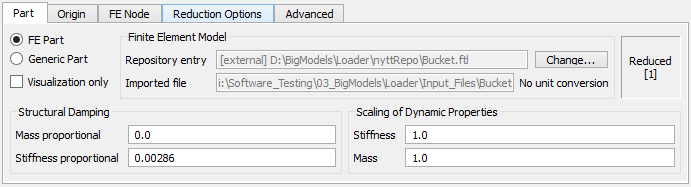
\includegraphics[width=\textwidth]{\ReferenceImg/prp/part-1}}
    \put(-8,64){\Bullet{1}}
    \put(-8,47){\Bullet{2}}
    \put(117,69){\Bullet{3}}
    \put(317,67){\Bullet{4}}
    \put(67,32){\Bullet{5}}
    \put(267,32){\Bullet{6}}
  \end{picture}
\end{figure}

\begin{figure}[H]
  \begin{picture}(343,93)
    \put(0,0){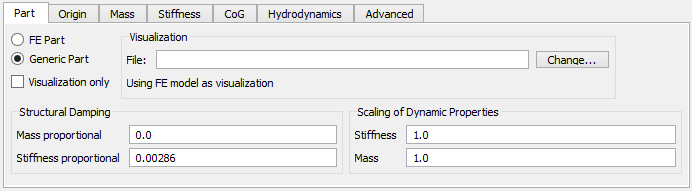
\includegraphics[width=\textwidth]{\ReferenceImg/prp/part-2}}
    \put(-8,64){\Bullet{1}}
    \put(67,32){\Bullet{5}}
    \put(267,32){\Bullet{6}}
    \put(117,69){\Bullet{7}}
  \end{picture}
\end{figure}

\begin{figure}[H]
  \begin{picture}(343,93)
    \put(0,0){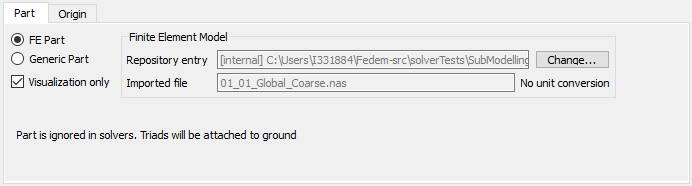
\includegraphics[width=\textwidth]{Figures/4-LinkPropPartTabVizOnly}}
    \put(-8,47){\Bullet{2}}
    \put(117,69){\Bullet{3}}
  \end{picture}
\end{figure}

\begin{bulletlist}
  \setlength\itemsep{1em}

\item{\sl FE Part/Generic Part} --
  Part type selector. You can switch between the FE model or the Generic Part
  model at any time during modeling.

\EnumNote{When switching between FE Part and Generic Part, Fedem tries
  to use the supplied FE data and visualization data in a sensible way.
  If your part is defined as an FE Part and you switch to Generic Part,
  the FE model is retained in memory and used as visualization
  unless a VRML model file is specified.
  Fedem will not drop the FE data from memory until you
  actively enter or change the VRML model file name.
  When switching back to FE Part,
  Fedem will check that all the Triads are validly attached to the FE model.
  See also \refSection{invalid-attachments}{Invalid attachments}.}

\item{\sl Visualization only} --
  You can define the part to be used for visualization only.
  The part will then be ignored by the solvers and actually serve as an
  extension of the {\sl Reference plane}
  (see \refSection{reference-plane}{Reference Plane}).
  The part and all triads attached to it will thus be {\sl grounded}.

\EnumNote{You can toggle a part as Visualization only at any time during
  modeling, but it is disallowed if the part has slave triads attached.}

\item{\sl Finite Element Model} (FE Parts only) --
  This group of options concerns the FE model used.

  \begin{itemize}
  \subitem{\sl Repository entry}
    indicates the repository type and the name of the selected \File{.ftl} file
    in the Fedem FE part repository
    (for details on the FE model repository, refer to
    \refSection{using-fe-model-repositories}{Using FE model repositories}).
    If the model file has not yet been saved, this entry will state
    the file name Fedem will use when you save your model.
  \subitem{\sl Imported file}
    indicates the name and location of the originally imported FE model file.
    The unit conversion that was applied during the import is also displayed.
  \subitem The \textbf{Change...} button
    allows you to replace the FE model of the part with a new one.
    This button opens a dialog box in which the new part file can be chosen.
    Note that all mechanism entities attached to the part, that do not have
    corresponding nodal points in the new FE model, will be detached.
  \end{itemize}

\item{\sl Needs reduction} (FE Parts only) --
  This label is a flag that signals if your FE model has been reduced or not.
  If some data for the reduced part is present and recognized to match the part,
  this entry will read {\sl Reduced [n]}, where {\sl n} is a number referring to
  the directory in the part database containing the reduced matrices.

\item{\sl Structural Damping} --
  Allows you to change the values of both the mass- and stiffness proportional
  damping for the part. These parameters are described in the
  \FedemTGuide{Section 7.5, "Structural damping"}.

\item{\sl Scaling of dynamic properties} --
  Allows you to scale stiffness and mass of each individual part
  in the dynamics simulation. The scaling is done during initialization
  and stays in effect for the entire analysis.
  This option is useful for sensitivity studies of deflection and stiffness.

\EnumWarning{The mass and stiffness scaling is not accounted for in any of the
  recovery analyses, and the recovered result will thus be misleading on
  FE parts using mass and/or stiffness scaling.}

\EnumWarning{The damping matrix and the associated force vector are not affected
  by the mass- and stiffness scaling parameters. That is, when using mass-
  and/or stiffness-proportional damping, it is the unscaled mass and stiffness
  matrix that contributes to the damping matrix and force vector.}

\EnumWarning{The mass- and stiffness scaling is not accounted for during FE part
  reduction. Therefore, the component mode shapes are always computed from the
  unscaled mass and stiffness matrix.
  Using stiffness and/or mass scaling on an FE part having component modes might
  thus yield incorrect results unless the two scaling factors are equal
  (because the component modes then are computed from a different
  set of matrices than the one used in the dynamics simulation).}

\item{\sl Visualization} {(Generic Parts only) --
  This frame contains options and information regarding the visualization
  of the Generic Part. The {\sl File} field can contain a path to a VRML file to
  use as a visualization for the Generic Part. Press the \textbf{Change...}
  button to browse for a file. If a valid FE model file is already referenced,
  Fedem will use that as a visualization until a VRML model file is specified.}
\end{bulletlist}


\SubSubSection{Origin tab}{origin-tab}

The {\sl Origin} tab is used to display and edit the position and
orientation of the part. See \refSection{origin-property}{Origin property}
for a description of the data fields in this tab.

\begin{figure}[H]
  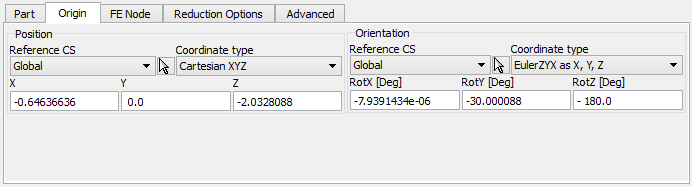
\includegraphics[width=\textwidth]{\ReferenceImg/prp/part-3}
\end{figure}


\clearpage
\SubSubSection{FE Node tab}{fe-node-tab}

The {\sl FE Node} tab is used to display information on FE nodes in
parts. If you click with the left mouse button anywhere on an FE part in
{\sl Modeler} view, the 3D Point Marker

\includegraphics[scale=0.7]{Figures/3d_point_marker}
will snap to the closest node and the node number and coordinates are
displayed in the Property Editor panel.

\begin{figure}[H]
  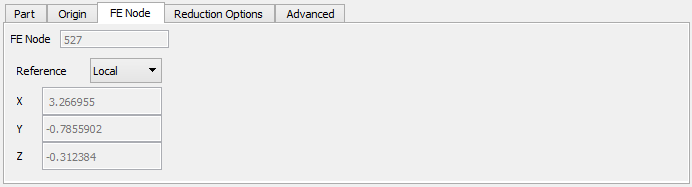
\includegraphics[width=\textwidth]{\ReferenceImg/prp/part-10}
\end{figure}


\SubSubSection{Reduction Options tab}{reduction-options-tab}

The settings on the {\sl Reduction Options} tab affect how the part is reduced.

\begin{figure}[H]
  \begin{picture}(343,93)
    \put(0,0){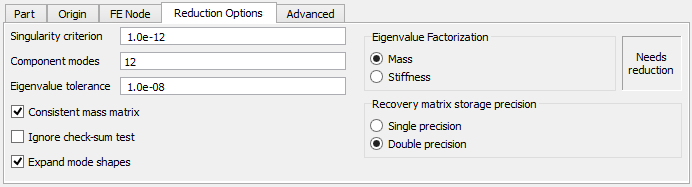
\includegraphics[width=\textwidth]{\ReferenceImg/prp/part-4}}
    \put(-10,71){\Bullet{1}}
    \put(-10,58){\Bullet{2}}
    \put(-10,45){\Bullet{3}}
    \put(-10,33){\Bullet{4}}
    \put(-10,21){\Bullet{5}}
    \put(-10,8){\Bullet{6}}
    \put(265,70){\Bullet{7}}
    \put(275,37){\Bullet{8}}
    \put(320,70){\Bullet{9}}
  \end{picture}
\end{figure}

\begin{bulletlist}
\item
  {\sl Singularity criterion} --
  This is the tolerance used to decide whether the stiffness and mass matrices
  are singular when they are factorized during model reduction. See
  \refSubSection{singularity-tolerance}{Singularity tolerance}
                {handling-singularities-during-the-model-reduction}.

\item{\sl Component modes} --
  Allows you to specify the number of component modes representing the internal
  (eliminated) nodal DOFs after CMS model reduction.
  See \refSection{using-component-modes}{Using component modes}.

\item{\sl Eigenvalue tolerance} --
  This is the maximum acceptable relative error in the computed eigenvalues
  in the fixed boundary eigenvalue analysis.

\item{\sl Consistent mass matrix} --
  Enables the use of consistent mass matrix in the model reduction process.
  If disabled, a lumped mass matrix approach is used.
  See \refSection{using-lumped-mass-matrix}{Using lumped mass matrix}.

\item{\sl Ignore check-sum test} --
  Disables the check on whether the reduced FE data, found in the FE model
  repository, is consistent with the part file currently used.
  Due to some rare numerical inconsistencies between reduced file data and the
  read FE data file, Fedem may signal that a part file needs reduction
  even though the reduced data are present.

\EnumCaution{Do not enable the Ignore check-sum test toggle unless you are sure
  that the reduced FE data found on disk are compatible with the current model.
  The consequence of using incompatible FE data may be a diverging model or
  incorrect results. A warning is issued whenever this toggle is enabled
  to stress this.}

\item{\sl Expand mode shapes} --
  Enables the expansion of component mode shapes and free-free mode shapes
  of the reduced part, for subsequent visualization. See
  \refSection{visualization-of-eigenmode-shapes-from-the-model-reduction}
             {Visualization of eigenmode shapes from the model reduction} and
  \refSection{animations}{Animations}.

\item{\sl Eigenvalue Factorization} --
  Allows you to specify which matrix to be Choleski-factorized during the
  eigenvalue analysis that is performed in the component modes computation.
  Default is the mass matrix.

\item{\sl Recovery matrix storage precision} --
  Allows you to switch to {\sl Single precision} storage of the recovery matrix
  (a.k.a. the B-matrix) on disk. This will reduce the needed disk space for this
  matrix by 50\%, and might be advantageous for very large parts with many
  triads that will result in a big B-matrix.
  The default is to use {\sl Double precision} storage.

\item{\sl Reduced/Needs reduction} --
  See \refSection{part-tab}{Part tab} above.
\end{bulletlist}

\Caution{Switching to single precision storage of the B-matrix should normally
  have no influence on the dynamics simulation results. However, if the part's
  FE model is poorly conditioned (e.g., there is a large span in the stiffness
  properties over the part) there may be minor loss of accuracy in the recovery
  results due to the truncation of the B-matrix elements stored on file.}

\Note{For parts that are reduced with component modes (see bullet 2 above),
  the single/double precision storage option also applies to the file
  containing the component mode shapes (the E-matrix file).}


\clearpage
\SubSubSection{Reduced Loads tab}{reduced-loads-tab}

On this tab you can assign time histories for load cases that are
defined in the FE data file. The associated reduced consistent load
vectors are computed by the Reducer and stored in the FE model
repository together with the reduced stiffness and mass matrices.

\begin{figure}[H]
  \begin{picture}(343,93)
    \put(0,0){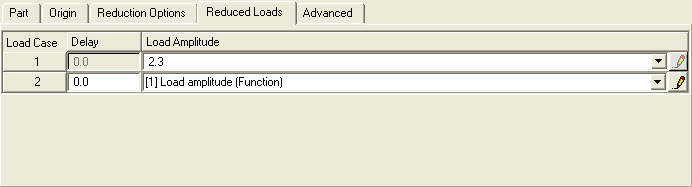
\includegraphics[width=\textwidth]{Figures/4-LinkPropRedLoads}}
    \put(10,35){\Bullet{1}}
    \put(40,35){\Bullet{2}}
    \put(100,35){\Bullet{3}}
  \end{picture}
\end{figure}

\begin{bulletlist}
\item{\sl Load Case } --
  This column contains the user-defined load case ID for each load set
  defined in the FE data file.

\item{\sl Delay} --
  If the load amplitude is defined by a Function, this value is used as a shift
  to the function argument, i.e., if the amplitude is specified as a function
  of time, $f(t)$, then the actual amplitude becomes $f(t-\mbox{\sl Delay})$.
  This is useful when each load case define the load state at different times
  in a transient simulation. The {\sl Delay} can then be set equal to the time
  where each load case is active, and the same function can then be applied to
  each load case to obtain a smooth transition from one load case to the next.

\item{\sl Load Amplitude} --
  You can either enter a constant value or select a Function
  (or Time history input file) from the pull-down menu.
  This value or function will then be used as a scaling of the reduced
  load vector associated with this load case in the dynamics simulation.
\end{bulletlist}


\clearpage
\SubSubSection{CoG tab}{cog-tab}

On this tab you can edit the position of the centre of gravity for a
Generic Part. You can also enter the orientation of the principal axis of
inertia to be used as the reference for the inertias entered on the
\refSection{mass-tab}{Mass tab}.

\begin{figure}[H]
  \begin{picture}(343,85)
    \put(0,-5){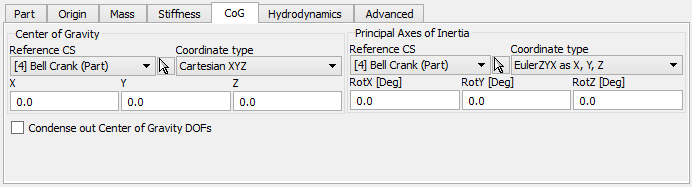
\includegraphics[width=\textwidth]{\ReferenceImg/prp/part-8}}
    \put(105,20){\Bullet{1}}
  \end{picture}
\end{figure}

\begin{bulletlist}
\item
  This toggle enables the elimination of the DOFs associated with the
  centre of gravity in the dynamics simulation. It is used to remove
  potential artificial internal vibrations in the Generic Part, and thus
  increase the numerical stability of the model.
\end{bulletlist}


\SubSubSection{Mass tab}{mass-tab}

The settings on this tab concern the mass and inertia properties of a
Generic Part, and is used to establish the part's mass matrix
(see the \FedemTGuide{Section A.16, "Generic Part element"}).

\begin{figure}[H]
  \begin{picture}(343,90)
    \put(0,0){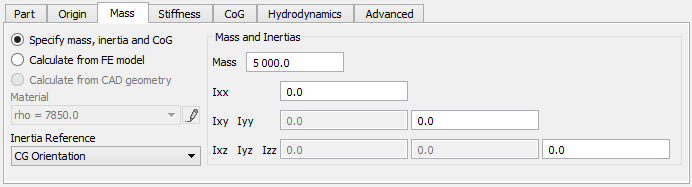
\includegraphics[width=\textwidth]{\ReferenceImg/prp/part-6}}
    \put(170,57){\Bullet{1}}
    \put(210,43){\Bullet{2}}
    \put(85,68){\Bullet{4}}
    \put(85,58){\Bullet{5}}
    \put(85,48){\Bullet{6}}
    \put(57,10){\Bullet{3}}
    \put(42,31){\Bullet{7}}
  \end{picture}
\end{figure}

\begin{bulletlist}
\item{\sl Mass} --
  The total mass of the part.

\item{\sl Ixx - Izz} --
  Lower triangle of the inertia matrix at the centre of gravity.

\item{\sl Inertia Reference} --
  Select whether to specify the inertia in the directions of the part coordinate
  system or in the directions specified as {\sl Principal Axes of Inertia}
  on the \protect\hyperlink{cog-tab}{\sl CoG tab}.

\item{\sl Specify mass, inertia and CoG} --
  The part mass and inertias must be specified explicitly in the
  {\sl Mass and Inertias} fields of this tab.
  The centre of gravity must also be specified in the
  \protect\hyperlink{cog-tab}{\sl CoG tab}.

\item{\sl Calculate from FE model} --
  The part mass and inertias, as well as the centre of gravity in the
  \protect\hyperlink{cog-tab}{\sl CoG tab},
  will be calculated from the FE model associated with the part.
  The {\sl Inertia Reference} will also be set to {\sl Part Orientation}
  and editing of the {\sl Mass and Inertia} fields are disabled.

\item{\sl Calculate from CAD geometry} --
  The mass, inertias, and the centre of gravity of the part will be calculated
  from the {\sl Visualization} file associated with it, and the chosen
  {\sl Material}. The {\sl Inertia Reference} will also be set to
  {\sl Part Orientation} and editing of the {\sl Mass and Inertia}
  fields are disabled.

\item{\sl Material} --
  If the {\sl Calculate from CAD geometry} toggle is enabled,
  you can select the material object from which the mass density to be used in
  the mass property calculation is taken. If no material object is selected,
  the value 7850.0 is used (appropriate for steel materials).
\end{bulletlist}


\SubSubSection{Stiffness tab}{stiffness-tab}

The stiffness properties of a Generic Part can be controlled on this tab.

\begin{figure}[H]
  \begin{picture}(343,90)
    \put(0,0){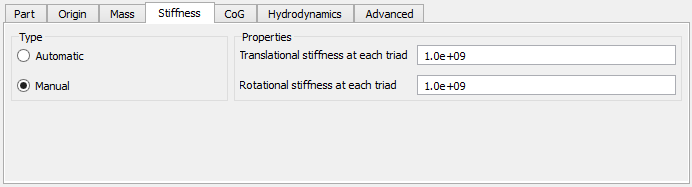
\includegraphics[width=\textwidth]{\ReferenceImg/prp/part-7}}
    \put(30,70){\Bullet{1}}
    \put(145,69){\Bullet{2}}
  \end{picture}
\end{figure}

\begin{bulletlist}
\item{\sl Type} --
  These radio buttons choose whether to set the overall Generic Part stiffness
  manually, or to have Fedem calculate a near rigid stiffness for you.

\item{\sl Properties} --
  This frame contains values for the manually selected stiffnesses.
\end{bulletlist}

When setting the stiffness calculations to {\sl Automatic}, Fedem uses the mass
and a high target eigen frequency to calculate a sensible high stiffness.
This will work as long as the mass of the part is set to something sensible.
Thus Fedem is not able to calculate a good stiffness for a part with no mass at
all, or with a mass that does not correspond to the actual use of the part.
In such cases you will need to set the stiffness manually.

See the \FedemTGuide{Section A.16, "Generic part element"}
for details on how the Dynamics Solver derives a part stiffness matrix
from the manually specified stiffness values.


\SubSubSection{Hydrodynamics tab}{hydrodynamics-tab}

This tab concerns the calculation of hydrodynamic forces on a part.

\begin{figure}[H]
  \begin{picture}(343,93)
    \put(0,0){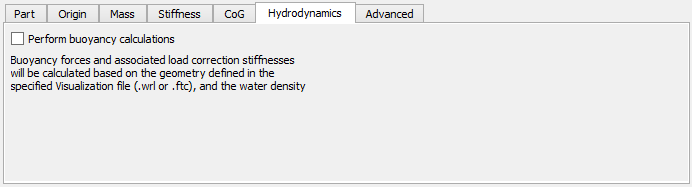
\includegraphics[width=\textwidth]{\ReferenceImg/prp/part-9}}
    \put(-12,68){\Bullet{1}}
  \end{picture}
\end{figure}

\begin{bulletlist}
\item{\sl Perform buoyancy calculation} --
  Enables the calculation of buoyancy forces for this part, provided a geometry
  description file has been specified in the {\sl Visualization} field of the
  \protect\hyperlink{part-tab}{\sl Part tab}. This geometry file has to define
  a closed volume that represents the total displaced fluid body when the part
  is submerged. It can be either on the VRML-format, or the Fedem Technology
  Cad format (\File{.ftc}).
\end{bulletlist}


\SubSubSection{Advanced tab}{advanced-tab}

This tab contains drop-down menus and toggles for selection of some advanced
settings that will apply during the dynamics simulation for the selected part.

\begin{figure}[H]
  \begin{picture}(343,93)
    \put(0,0){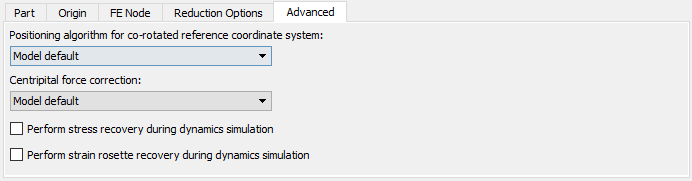
\includegraphics[width=\textwidth]{\ReferenceImg/prp/part-5}}
    \put(140,57){\Bullet{1}}
    \put(140,35){\Bullet{2}}
    \put(-10,15){\Bullet{3}}
  \end{picture}
\end{figure}

\begin{bulletlist}
\item The options for the {\sl co-rotated reference coordinate system} are:
  \begin{itemize}
  \subitem{\sl Model default} : The global setting defined in the
    \protect\hyperlink{integration-tab}{\sl Integration tab} of the
    Dynamics Solver Setup is used (see
    \refSection{dynamics-solver-advanced-mode}{Dynamics Solver (Advanced Mode)}).
  \subitem{\sl Max triangle, with unit offset when necessary} :
    This is the original algorithm, the only one available in Fedem R3.1.1
    and earlier.
  \subitem{\sl Max triangle, with scaled offset when necessary} : Same as above,
    but with adjustments of the offset to better fit the part size.
  \subitem {\sl Mass based nodal average} :
    Algorithm based on equilibrium of a rigid shadow element with averaged
    stiffnesses at the triads.
  \end{itemize}

  See the \FedemTGuide{Section 4.1, "Superelement local coordinate system"}
  for a detailed description of these algorithms.

\item The options for the {\sl centripetal force correction} are:
  \begin{itemize}
  \subitem{\sl Model default} : The global setting defined in the
    \protect\hyperlink{integration-tab}{\sl Integration tab} of the
    Dynamics Solver Setup is used (see
    \refSection{dynamics-solver-advanced-mode}{Dynamics Solver (Advanced Mode)}).
  \subitem{\sl On} : Turns centripetal force correction on for this part.
  \subitem{\sl Off} : Turns centripetal force correction off for this part.
  \end{itemize}

\item These two toggles enable/disable
  the calculation of internal deformations and stresses/strains in,
  respectively, the finite elements and strain rosette elements in the FE part
  during the dynamics simulation, see
  \refSection{stress-and-strain-recovery-during-time-integration}
             {Stress and strain recovery during time integration}.
\end{bulletlist}


\SubSection{Using FE model repositories}{using-fe-model-repositories}

A FE model repository is a directory structure containing all the files
related to one or more FE parts. This includes the FE model files,
reducer input option files, the reduced matrix and load files, the
displacement recovery matrix files, and log-files with text-based output
from the model reduction processes.

The term part database is also used when referring to a FE model repository.
For detailed information about part databases,
see \refSection{part-database}{Part database}.

Fedem can handle FE model repositories in three different ways:

\begin{itemize}
\item{\sl Internal repository} (default) --
  The default FE model repository is placed inside the model results database
  in the \File{link\_DB/} directory. This repository will follow the model,
  and be copied along with the results if saving the model as a new name.
\item{\sl External repository} --
  Sometimes it is useful to be able to share and reuse the FE model repository
  among several model files. Using an external repository enables such sharing.
  If this is set, using \textbf{Save As ...} will not copy the FE model
  repository, but the original and the new model will point to the same
  repository and thus share any identical information.
\item{\sl External single part repository} --
  It is possible to use a specific FE model repository for an individual part.
  This is used to import and reuse a part from an existing FE model repository.
\end{itemize}


\SubSubSection{Setting the FE model repository}{setting-the-fe-model-repository}

The FE model repository can be set in the Model Preferences dialog box (see
\refSection{model-preferences}{Model preferences}).
Select \textbf{Model Preferences...} from the \textbf{Edit} menu to open it.
Below is a portion of that dialog box shown.

\begin{figure}[H]
  \center
  \begin{picture}(258,50)
    \put(0,0){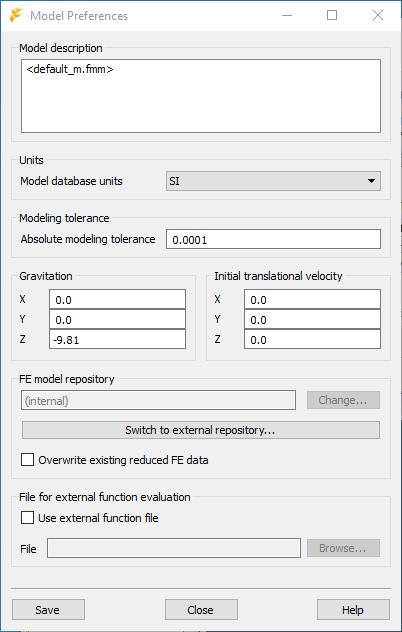
\includegraphics[trim=0 135 0 271,clip,width=0.75\textwidth]{\ReferenceImg/dlg-model-preferences}}
    \put(130,28){\Bullet{1}}
    \put(230,29){\Bullet{3}}
    \put(230,9){\Bullet{2}}
  \end{picture}
\end{figure}

\begin{bulletlist}
\item Path to the current FE model repository, unless {\tt(internal)}.
\item This button switches between internal and external repository.
\item The \textbf{Change...} button
  changes the external repository to a new directory.
  This might be an empty directory, or a directory used as FE model repository
  by another model.
\end{bulletlist}

When changing the repository, Fedem will copy the active content of the
current repository to the new destination prompting on whether to
overwrite if necessary. The old repository will be left untouched,
unless it is an internal repository. Internal repositories will be
deleted when switching to an external repository.

If there exists files with the same names at the new destination, Fedem
will try to find out whether the reduced data match the existing FE model.
If it does the reduced data will not be copied, as identical data is assumed to
exist at the new destination.


\subsubsection{Reusing a part from an existing FE model repository}

To import and reuse the reduced data for a part, the part can be imported from
the existing FE model repository using the \textbf{Load Part...} command.
See \refSection{creating-parts-by-file-import}{Creating parts by file import}.
Select the \File{.ftl} file you want, and toggle on the
{\sl Use part-specific repository} toggle in the Load Part dialog box.
You will then need to add triads and reducer options for that particular part,
that match the options and triad positions used by the previously reduced part.
When done, Fedem will detect the reduced files,
and flag the part as {\sl Reduced}.
